\providecommand{\main}{..}
\documentclass[\main/main.tex]{subfiles}


\begin{document}


\section{MOSFET}
\subsection{NMOS ed PMOS}
Esistono due tipi duali e complementari di MOSFET: NMOS (Piu' usati e con caratteristiche migliori) e i PMOS.

Definisco due costanti:

\[K_n = \frac{1}{2} \mu_n C_{ox}'\left(\frac{W}{L}\right)\]
\[K_n' = \frac{1}{2} \mu_n C_{ox}'\]
\begin{align*}
\mu_n &\text{ e' la costante di mobilita' degli elettroni}\\
C_{ox}' &\text{ e' la capacita' del condesatore che si forma tra il gate ed il canale}\\
W &\text{ e' la larghezza del canale}\\
L &\text{ e' la lunghezza del canale}
\end{align*}
quindi $K_n = K_n' \left(\frac{W}{L}\right)$

\clearpage
\subsubsection{NMOS}

\begin{center}
\begin{circuitikz} \draw
(0,0) node[nmos] (mos) {}
(mos.gate) node[anchor=east] {G}
(mos.drain) node[anchor=south] {D}
(mos.source) node[anchor=north] {S}
;\end{circuitikz}
\end{center}
Il NMOS e' spento se la $V_{GS} < V_t$

e quindi la corrente
 \[I_{DS} = 0\]


Il NMOS e' in regime ohmico o lineare se $V_{DS} < V_{GS} - V_t$

e quindi la corrente 

\[I_{DS} = K_n \left[ 2 \left(V_{GS} - V_t \right)V_{DS} - V_{DS}^2 \right]\]


Il NMOS e' in zona di saturazione se $V_{DS} > V_{GS} - V_t$

e quindi la corrente 

\[ I_{DS} = K_n \left( V_{GS} - V_t \right)^2\]

\begin{center}
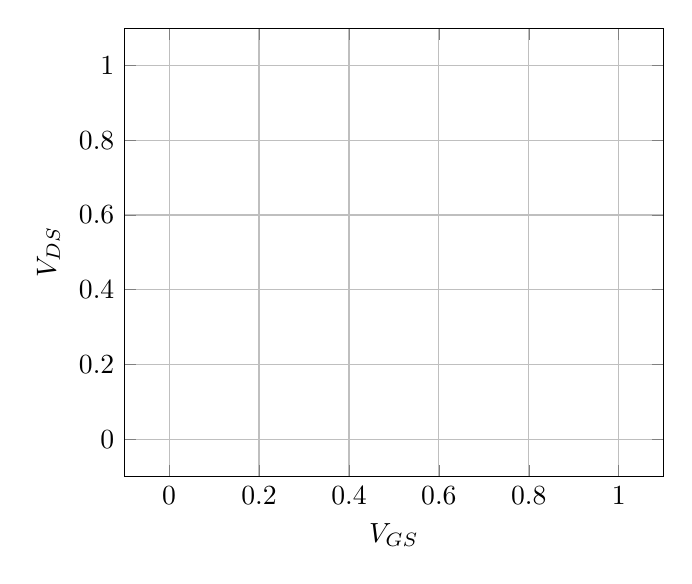
\begin{tikzpicture}
\begin{axis}[
 grid=major,
 samples=\samples,
 xlabel=$V_{GS}$,
    ylabel=$V_{DS}$,
    ]
   \draw [green,domain=0:2*pi] plot (\x, {(sin(\x r)* ln(\x+1))/2});
\end{axis}
\end{tikzpicture}
\end{center}

\begin{center}
\begin{tikzpicture}
\begin{axis}[
 grid=major,
 samples=\samples,
 xlabel=$V_{GS}$,
    ylabel=$V_{DS}$,
    zlabel=$I_{DS}$
]

\addplot3[surf, unbounded coords=jump]
{x^2 + y^2 > 4 && x < 3/2 ? (x-1)^2 + y^2 : NaN};

\end{axis}
\end{tikzpicture}
\end{center}

INSERIRE QUI GRAFICI I/VDS I/VGS VDS/VGS
\clearpage
\subsubsection{PMOS}


\begin{center}
\begin{circuitikz} \draw
(0,0) node[pmos] (mos) {}
(mos.gate) node[anchor=east] {G}
(mos.drain) node[anchor=north] {D}
(mos.source) node[anchor=south] {S}
;\end{circuitikz}
\end{center}
ATTENZIONE AI SEGNI

Il PMOS e' spento se la $\left|V_{GS}\right| < \left|V_t\right|$

e quindi la corrente
 \[I_{SD} = 0\]


Il PMOS e' in regime ohmico o lineare se $V_{SD} < V_{SG} - |V_t|$

e quindi la corrente 

\[I_{SD} = K_p \left[ 2 \left(V_{GS} - |V_t| \right)V_{SD} - V_{SD}^2 \right]\]


Il PMOS e' in zona di saturazione se $V_{SD} > V_{GS} - |V_t|$

e quindi la corrente 

\[ I_{SD} = K_p \left( |V_{GS}| - |V_t| \right)^2\]

\clearpage

\subsection{Come capire in che stato di funzionamento e' il MOSFET}
Prendiamo un NMOS per comodita'.
Metodo dei Diodi:

\begin{center}
\begin{circuitikz} \draw
(0,0) node[nmos] (mos) {}
(mos.gate) node[anchor=east] {G}
(mos.drain) node[anchor=south] {D}
(mos.source) node[anchor=north] {S}
;\end{circuitikz}
\end{center}

Il Mosfet essendo in fondo una giunzione NPN e' approssimabile a due diodi in antiserie.
Quindi sostanzialmente ci sono 3 fasi di funzionamento del MOSFET: Off,Ohm,Sat (Spento,Ohmmica,Saturazione).

Off e' quando non vi e' canale da nessuno dei due lati.

Ohm e' quando vi e' canale da entrambi i lati.

Sat quando vi e' canale da solo un lato.

Le regole normali sono:

Se la tensione $V_{GS} < V_t$ allora il MOSFET e' Off

Altrimenti se  $V_{DS} < V_{GS} - V_t$ Il MOSFET e' Ohm

Ed in fine se  $V_{DS} > V_{GS} - V_t$ Il Mosfet e' Sat

Ora osserviamo che
\[V_{DS} < V_{GS} - V_t\]
\[V_{DS} - V_{GS} <  - V_t\]
\[-V_{GS} <  - V_t\]
\[V_{DG} > V_t\]

quindi se $V_{GS} < V_t$ allora vi e' canale dal lato del Source

e se $V_{DG} > V_t$ allora vi e' canale dal lato del Drain

ora se sono entrambe vere si e' in zona Ohmmica, se una sola delle due e' vera si e' in Saturazione, quando sono entrambe false il MOSFET e' spento.


Metodo Grafico :
Basta seguire 4 punti:

$(1)$ Verificare che la $V_{GS} > V_t$

$(2)$ Calcolare la corrente $I_{DS}$ del NMOS quando $V_{DS} = V_{ow} = V_{GS} - V_{t}$

$(3)$ Calcolare le correnti ad un nodo a scelta tra SOURCE e DRAIN imponendo che $V_{DS} = V_{ow}$

$(4)$ Confrontare i due valori.

Se la corrente del NMOS e' maggiore della somma di quelle del nodo allora il NMOS e' in zona ohmmica.

Altrimenti Se la somma delle correnti del nodo e' maggiore di quella del NMOS allora esso e' in saturazione.

Dimosrazione:

QUA METTI GRAFICI BELLI PLZ

\subsection{Caratteristiche Importanti dei MOSFET}
\textbf{Tensione di Overdrive $V_{ow}$}
\[ V_{ow} = V_{GS} - V_t\]
e' utile per scrivere le formule in modo piu' compatto.

\textbf{Tensione di soglia logica $V_{th}$}
\[V_{th} \triangleq V \text{ t.c. } V_{in} = V_{out}\]

\textbf{Potenza Statica $P_{STAT}$}
Sono le potenze consumate dalla porta per rimanere in ogni suo stato.

\textbf{Potenza Statica $P_{DIM}$}
Sono le potenze consumate dalla porta per commutare da stato a stato.

\textbf{Tempo di propagazione $t_p$}
Il Tempo di propagazione e' quanto ci mette la porta a fare da 0\% al 50\% della sua escurisione di tensione.
Vi sono due approssimazioni usabili per calcolarla:

$(1)$ Approssimazione a corrente costante
In questa approssimazione si considera il mosfet sempre in saturazione, questa approssimazione di solito sottostima del 10\%.
\[ I_{DS} = K_n \left( V_{GS} - V_t \right)^2\]

$(2)$ Approssimazione a Resistenza
In questa approssimazione si approssima il mosfet ad una resistenza di resistivita', questa approssimazione di solito sovrastima.
\[R_{eq} = \frac{V_f}{I_{sat}} \]
Comunque una volta decisa l'approssimazione si calcola la corrente del condensatore $I_c$ poi si calcola il delta di carica che serve per caricare il condensatore:
\[Q_i = C V_i\]
\[Q_f = C V_f\]
\[\bigtriangleup Q = Q_f - Q_i = C \left( V_f - V_il\right) \]
a questo punto vale la relazione:
\[I_c = \frac{\bigtriangleup Q}{t_p}\]
e si ricava $t_p$:
\[t_p = \frac{\bigtriangleup Q}{I_c} = C \frac{V_f - V_i}{I_c}\]



\subsection{Tips and Tricks}
$(1)$ I MOSFET sono simmetrici e quindi non ha senso parlare di Source e Drain pero' per aiutare convenzione si ha che:

La corrente nei MOSFET scorre sempre in senso concorde alla freccia.

La tensione $V_{GS}$ si misura sempre tra il piedino dove vi e' la freccia e il gate ed ha sempre senso contrario alla freccia.

In pratica queste sono convenzioni per suggerire il funzionamento del MOSFET a chi sta studiando il circuito.

$(2)$ Per Piccole $V_{DS}$ si puo' approssimare:

\[I_n = K_n \left[ 2 \left( V_{GS} -V_t \right)V_{DS} - V_{DS}^2 \right] \sim K_n \left[ 2 \left( V_{GS} -V_t \right)V_{DS} \right]\]
Poiche' se $V_{DS}$ e' piccolo $V_{DS}^2$ e' ancora piu' piccolo e quindi si puo' trascurare senza grossi problemi.

La quale e' una equazione lineare e quindi piu' semplice da risolvere.

Per esempio sul circuito del esercizio 1 con la equazione corretta si ottiene 

$V_r = 0.1416V$

mentre con la seconda equazione si ottiene

$V_r = 0.1435V$


\clearpage
\subsection{Come Risolvere gli esercizi sui MOSFET}
\subsubsection{Esercizio 1}
Dato il Circuito sottostante Calcolare $V_{out}$ nei casi 
$(a)$ $V_{in} = 0V$
$(b)$ $V_{in} = 3.3V$

Poi si calcoli Soglia logica $V_{th}$, Potenza Statica $P_{STAT}$.


\begin{center}
\begin{circuitikz}
\draw (0,-3)
 node[nmos] (mos) {}
(mos.gate) node[anchor=east] {G,$V_{in}$}
(mos.drain) node[anchor=south,xshift=-0.25cm] {D}
(mos.source) node[anchor=north,xshift=-0.25cm] {S};
\draw (0,0)
node[vcc]{3.3V}
to[R=$R$,v<=$V_r$,i=$i_r$] (0,-2)
-- (mos.drain);
\draw (mos.source)
node[ground] {Gnd} (0,-4);
\draw (mos.drain)
to[short, *-] (1,-2.25)
to[short] (1,-2.50)
to[C=$C_l$,v<=$V_{out}$] (1,-3.50)
to[short] (1,-4)
to[short] (0,-4)
;
\end{circuitikz}
\end{center}

Dati:

\[V_{cc} = 3.3V\]
\[R = 1k\Omega\]
\[K_n = 5 \frac{mA}{V^2}\]
\[|V_t| = 1V\]
\[C_l = 10pF\]
\subsubsection{Risoluzione Esercizio 1}
$(a)$ $V_{in} = 0V$

poiche' sia $V_{in}$ che la tensione al SOURCE allora la tensione $V_{GS} = V_G - V_S = 0$ quindi l'NMOS e' spento quindi $I_n = 0$ e poiche' il NMOS si comporta come circuito aperto anche la corrente della resistenza $I_r = I_n = 0$ e di conseguenza anche la caduta di tensione sulla resistenza e' $0$ poiche' la sua eq caratteristica e' $V = RI$ quindi non essendoci caduta di tensione sulla resistenza $V_{out} = V_{cc} = 3.3V$.

Quindi:
 \[V_{in} = 0V \Rightarrow V_{out} = 3.3V\]
 

$(b)$ $V_{in} = V_{GS} = 3.3V$

quindi $V_{ow} = |V_{GS}| - |V_t| = 2,3V$ quindi $V_{GS} > V_t$ quindi l'NMOS e' Acceso.
Ora bisogna stabilire se si trova in regime ohmmico o di saturazione e procediamo per metodo grafico:

$(1)$ Calcoliamo la corrente $I_{DS}$ quando $V_{DS} = V_{ow}$ e possiamo usare una qualunque tra le due equazioni poiche' in corrispondenza di $V_{ow}$ si raccordano entrambe nello stesso punto, quindi usiamo quella in regime di saturazione poiche' piu' semplice.

\[I_n|_{ow} = K_n \left(V_{ow}\right)^2 = 26mA\]

$(2)$ Calcoliamo la corrente del carico $I_{L} = I_{R}$ che in questo caso coincide con quella della resistenza.

\[I_R|_{ow} = \frac{V_{cc} - V_{ow}}{R} = 1mA\]

$(3)$ Ora si confrontano le due correnti:

Poiche' $I_n|_{ow} = 26mA > I_R|_{ow} = 1mA$ ci si trova in zona Ohmmica, nel caso opposto sarebbe in saturazione.

Quindi ora si calcola $V_{DS}$ Col bilancio delle correnti $I_R = I_n$

\[\frac{V_{cc} - V_{DS}}{R} = K_n \left[ 2 \left(V_{GS} - V_t \right)V_{DS} - V_{DS}^2 \right]\]

Che e' una equazione di secondo grado in $V_{DS}$ 

\[\left(K_n R \right) V_{DS}^2 - \left(2K_nR\left(V_{GS}-V_t\right)+1\right)V_{DS}+V_{cc} = 0\]

La quale parabola ha come radici:

\[V_{DS1} = 4.6V\]
\[V_{DS2} = 0.14V\]

Ovviamente ci puo' essere un solo valore vero, quindi uno e' da scartare.
In questo caso Poiche' $V_{DS1} > V_{cc}$ e $V_{DS1} > V_{ow}$ ci porta a scartare $V_{DS1}$

Quindi $V_{DS} = V_{DS2} = 0.14V$

E poiche' $V_{out} = V_{DS}$ allora $V_{out} = 0.14V$

E quindi in sinossi:

\[V_{in} = 3.3V \Rightarrow V_{out} = 0.14V\]

Calcolo della soglia logica $V_{th}$:

La soglia logica e' la tensione che separa la zona che consideriamo ON da quella che consideriamo OFF.

L'ideale sarebbe $V_{th} = \frac{V_{cc}}{2}$

\[V_{th} = \frac{\bigtriangleup V}{2} = \frac{\left | V_{on} - V_{off} \right |}{2} = \frac{3.3V - 0.14V}{2} = 1.58V\]

Calcolo Delle Potenze Statiche $P_{STAT}$:

In questo circuito abbiamo due potenze statiche, quando la porta e' ON e quando e' OFF.

Caso ON $V_{in} = 0V$:

\[P_{STAT,On} = V_{cc} I_{n} = 0W\]
Poiche' non scorre corrente, il consumo di corrente e' 0 watt. Ottimo.


Caso OFF $V_{in} = 3.3V$:

$P_{STAT,Off} = V_{cc} I_{n} = 3.3V * I_{n}$

coi dati prima calcolati possiamo ricavare $I_{n}$

\[I_{n} = I_{r} = \frac{V_{cc} - V_{DS}}{R} = \frac{3.3V - 0.14V}{1k\Omega} = 3.16mA\]
\[P_{STAT,Off} = V_{cc} I_{n} = 3.3V * 3.16mA = 10,4mW\]
Un consumo veramente grande per una porta cosi piccola. SI puo' fare di meglio.

\clearpage
\subsubsection{Esercizio 2}
Dato il Circuito sottostante Calcolare $V_{out}$ nei casi 
$(a)$ $V_{in} = 0V$
$(b)$ $V_{in} = 3.3V$

Poi si calcoli Soglia logica $V_{th}$, Potenza Statica $P_{STAT}$, Potenza Dinamica $P_{DIN}$, e tempo di propagazione $t_p$.



Dati:

\[V_{cc} = 3.3V\]
\[R = 1k\Omega\]
\[C = 1pF\]
\[|K_p| = 2 \frac{mA}{V^2}\]
\[|V_t| = 1V\]
\subsubsection{Risoluzione Esercizio 2}
$(b)$ $V_{in} = 3.3V$

Poiche' $V_{cc} = V_{in} = 3.3V$ allora $V_{SG} = V_{cc} - V_{in} = 0V$ e 
$V_{SG} < |V_t|$ quindi il PMOS e' spento! Quindi $I_p = I_{SD} = 0A$ ora con una KCL al nodo del DRAIN otteniamo che $I_p = I_r + I_c$ quindi $I_r + I_c = 0$ ora poiche' l'eq caratteristica del condensatore e' $i_c(t) = C \frac{d}{dt}V_c$ e si suppone sempre che i transitori siano finiti allora il condensatore e' scarico $V_c = 0$ e quindi la sua corrente $I_c = 0$, il che implica che $I_r + I_c = I_r = 0$ e quindi la tensione $V_r = R I_r = 0$ e di conseguenza: $V_{out} = V_c = V_r = 0V$.

\[V_{in} = 0V \Rightarrow V_{out} = 0V\]

$(a)$ $V_{in} = 0V$

$V_{SG} = V_{in} - V_{cc} = -3.3V$ e $|V_{SG}| > |V_t|$ e $V_{ow} = |V_{SG}| - |V_t| = -2.3V$ quindi il PMOS e' Acceso.
Ora bisogna stabilire in che zona di lavoro sia, procediamo per metodo grafico.

$(1)$ Calcoliamo la corrente del PMOS alla tensione di overdrive $V_{ow}$:

\[I_p |_{ow} = K_p \left(V_{ow}\right)^2 = 10.58mA\]

$(2)$ Calcoliamo la corrente di carico assumendo che $V_{DS} = V_{ow}$

Poiche' la resistenza ed il condensatore sono in parallelo $V_r = V_c$ e cosi con una KVL si ottiene che $V_r = V_c = V_{cc} - V_{DS} = 1V$ poiche' si calcola in condizioni di regime Il condensatore e' completamente carico a $V_c = 1V$  e quindi come sopra poiche' il consensatore e' carico la sua corrente $I_c = 0$.

Quindi dalla KCL al nodo del DRAIN la corrente \[I_{DS}|_{ow} = I_r + I_c = I_r = \frac{V_r}{R}= \frac{ V_{cc} - V_{ow}}{R} =  \frac{ V_{cc} - V_{cc} + V_t}{R} = \frac{V_t}{R} = 1mA\]

$(3)$ Confrontando le due correnti $I_{DS}|_{ow} = 1mA < I_p |_{ow} = 26mA$ quindi il PMOS si trova in zona Ohmmica.


Stabilito cio' si calcola il punto di lavoro col bilancio delle correnti:
$I_r = I_{DS,Ohm}$

\[\frac{V_{cc} - |V_{SD}|}{R} = K_p \left[ 2 \right(|V_{GS}| - |V_t|)V_{SD} - V_{SD}^2\]
e quindi otteniamo una equazione di secondo grado in $V_{SD}$ che risolvendola ha come soluzioni:

$V_{SD1} = 4.75V$ che scarteremo poiche' $V_{SD1} > V_{cc}$ e $V_{SD1} > |V_{GS}| - |V_t|$ quindi dovrebbe essere in saturazione quando abbiamo gia' dimostrato che e' in zona ohmmica.

e

$V_{SD2} = V_{SD} = 0.347V$ che e' la soluzione corretta.

Ora concludiamo con una KVL dalla quale si ottiene $V_{out} = V_{cc} - V_{SD} = 2.96V$

In Sinossi:
\[V_{in} = 0V \Rightarrow V_{out} = 2.96V\]
.

\end{document}